\documentclass{standalone}

\usepackage{lmodern}
\usepackage{tikz}
    \usetikzlibrary{positioning}

\begin{document}
    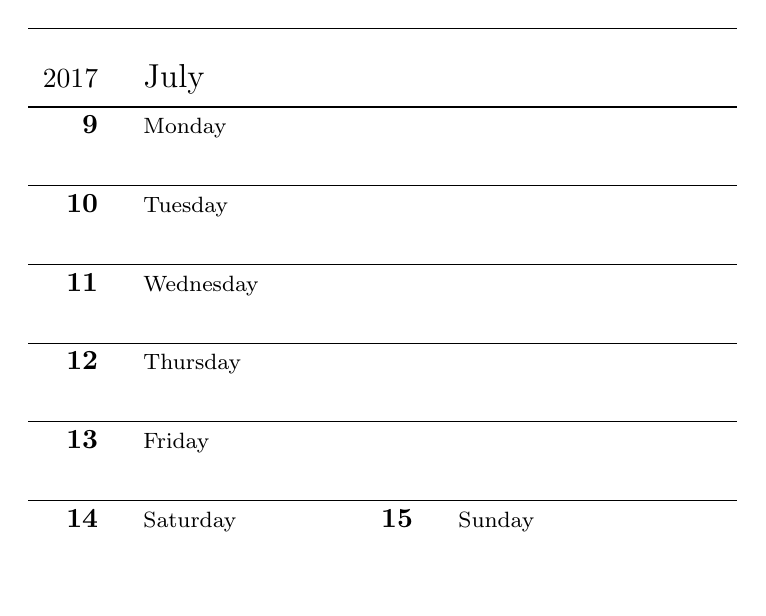
\begin{tikzpicture}[%
        inner sep=3 pt,
        dayname/.style={%
            node font=\footnotesize, 
        },
        daynumber/.style={%
            anchor=north east,
            node font=\normalsize\bfseries, 
        },
        xscale = 4,
        yscale=-1,
    ]

    \node (saturday_number) at (0,6) [daynumber] {14};
    \node [base right = 1em of saturday_number, anchor=base west] [dayname] {Saturday};

        \node (sunday_number) at (1,6) [daynumber] {15};
        \node [base right = 1em of sunday_number, anchor=base west] [dayname] {Sunday};

    \node (friday_number) at (0,5) [daynumber] {13};
    \node [base right = 1em of friday_number, anchor=base west] [dayname] {Friday};

    \node (thursday_number) at (0,4) [daynumber] {12};
    \node [base right = 1em of thursday_number, anchor=base west] [dayname] {Thursday};

    \node (wednesday_number) at (0,3) [daynumber] {11};
    \node [base right = 1em of wednesday_number, anchor=base west] [dayname] {Wednesday};

    \node (tuesday_number) at (0,2) [daynumber] {10};
    \node [base right = 1em of tuesday_number, anchor=base west] [dayname] {Tuesday};

    \node (monday_number) at (0,1) [daynumber] {9};
    \node [base right = 1em of monday_number, anchor=base west] [dayname] {Monday};

    \node (year_number) at (0,1) [anchor = south east, minimum height = 2em] {2017};
    \node [base right = 1em of year_number, anchor=base west, node font=\large] {July};

    \foreach \i in {0,1,...,6} {%
        \draw (-0.25,\i) -- (2,\i);
    }

    \node (SW-corner) at (0,7) {};
    \end{tikzpicture}
\end{document}